%%%%%%%%%%%%%%%%%%%%%%%%%%%%%%%%%%%%%%%%%%%%%%%%%%%%%%%%%%%%%%%%%%%%%%%%%
% All the content is in one file because I do not expect multiple editors.
%%%%%%%%%%%%%%%%%%%%%%%%%%%%%%%%%%%%%%%%%%%%%%%%%%%%%%%%%%%%%%%%%%%%%%%%%

\documentclass[11pt]{article}

%%%%%%%%%%%%%%%%%%%%%%%%%%%%%%%%%%%%%%%%%%%%%%%%%%%%%%%%%%%%%%%%%%%%%%%%%
%% packages

\usepackage{latexsym}
\usepackage{algorithm}
\usepackage{algorithmic}
\usepackage{graphicx}
\usepackage{subfigure}
\usepackage[T1]{fontenc}
% \usepackage{mathptmx}
 \usepackage{newcent}
%\usepackage{fouriernc}
%\usepackage{times}
\usepackage{amsmath}
\usepackage{amssymb}
\usepackage{amsfonts}
\usepackage{fullpage}
% \usepackage{complexity}
\usepackage{hyphenat}
\usepackage{multirow}
\usepackage{empheq}
\usepackage{url}
\usepackage{enumitem}
\usepackage[lite, subscriptcorrection]{mtpro2}

\usepackage[mathscr]{euscript}

\usepackage{hyperref}
\hypersetup{
colorlinks = true
}

\makeatletter
\DeclareFontFamily{OMX}{MnSymbolE}{}
\DeclareSymbolFont{MnLargeSymbols}{OMX}{MnSymbolE}{m}{n}
\SetSymbolFont{MnLargeSymbols}{bold}{OMX}{MnSymbolE}{b}{n}
\DeclareFontShape{OMX}{MnSymbolE}{m}{n}{
    <-6>  MnSymbolE5
   <6-7>  MnSymbolE6
   <7-8>  MnSymbolE7
   <8-9>  MnSymbolE8
   <9-10> MnSymbolE9
  <10-12> MnSymbolE10
  <12->   MnSymbolE12
}{}
\DeclareFontShape{OMX}{MnSymbolE}{b}{n}{
    <-6>  MnSymbolE-Bold5
   <6-7>  MnSymbolE-Bold6
   <7-8>  MnSymbolE-Bold7
   <8-9>  MnSymbolE-Bold8
   <9-10> MnSymbolE-Bold9
  <10-12> MnSymbolE-Bold10
  <12->   MnSymbolE-Bold12
}{}

\let\llangle\@undefined
\let\rrangle\@undefined
\DeclareMathDelimiter{\llangle}{\mathopen}%
                     {MnLargeSymbols}{'164}{MnLargeSymbols}{'164}
\DeclareMathDelimiter{\rrangle}{\mathclose}%
                     {MnLargeSymbols}{'171}{MnLargeSymbols}{'171}
\makeatother


\renewcommand{\P}{\mathbb{P}}
\newcommand{\E}{\mathbb{E}}
\newcommand{\Q}{\mathbb{Q}}
\newcommand{\R}{\mathbb{R}}
\newcommand{\Z}{\mathbb{Z}}
\newcommand{\N}{\mathbb{N}}
\newcommand{\C}{\mathbb{C}}
\newcommand{\K}{\mathbb{K}}
\newcommand{\cA}{\mathscr A}
\newcommand{\cF}{\mathcal F}
\newcommand{\cB}{\mathscr B}
\newcommand{\cM}{\mathscr M}
\newcommand{\cG}{\mathscr G}
\newcommand{\cP}{\mathscr P}
\newcommand{\cL}{\mathscr L}
\newcommand{\cX}{\mathscr X}
\newcommand{\cZ}{\mathscr Z}
\newcommand{\cE}{\mathscr E}
\newcommand{\cN}{\mathscr N}
\newcommand{\cT}{\mathscr T}
\newcommand{\ran}{\text{ran}}
\newcommand{\dom}{\text{dom}}
\newcommand{\supp}{\text{supp}}
\newcommand{\eps}{\varepsilon}
\newcommand{\var}{\text{Var}}
\newcommand{\ind}{{\mathbf 1}}

%%%%%%%%%%%%%%%%%%%%%%%%%%%%%%%%%%%%%%%%%%%%%%%%%%%%%%%%%%%%%%%%%%%%%%%%%
%% basic definitions, environments

\newtheorem{theorem}{Theorem}
\newtheorem{lemma}{Lemma}
\newtheorem{corollary}[theorem]{Corollary}
\newtheorem{definition}{Definition}
\newtheorem{property}{Property}
\newtheorem{observation}{Observation}
\newtheorem{remark}{Remark}

\newenvironment{proof}
        {\noindent {\em Proof.}~~~} %\\
        {\begin{flushright}$\Box$\end{flushright}}

\addtolength{\oddsidemargin}{-0.25in}
\addtolength{\evensidemargin}{-0.25in}
\addtolength{\textwidth}{0.5in}
\addtolength{\topmargin}{-.25in}
\addtolength{\textheight}{0.75in}	


%%%%%%%%%%%%%%%%%%%%%%%%%%%%%%%%%%%%%%%%%%%%%%%%%%%%%%%%%%%%%%%%%%%%%%%%%
%% title details

\title{
  Written Assignment \#4 \\[0.5em]
  \large
  Vancouver Summer Program 2019 -- Algorithms -- UBC \\
  \vspace*{0.2in} \hrule
}

%\author{
%	Sathish Gopalakrishnan
%}

\date{}

%%%%%%%%%%%%%%%%%%%%%%%%%%%%%%%%%%%%%%%%%%%%%%%%%%%%%%%%%%%%%%%%%%%%%%%%%

\begin{document}

\maketitle

\setlength{\baselineskip}{0.90\baselineskip}

%%%%%%%%%%%%%%%%%%%%%%%%%%%%%%%%%%%%%%%%%%%%%%%%%%%%%%%%%%%%%%%%%%%%%%%%%
%% the abstract

%% no abstract needed

%%%%%%%%%%%%%%%%%%%%%%%%%%%%%%%%%%%%%%%%%%%%%%%%%%%%%%%%%%%%%%%%%%%%%%%%%

\pagestyle{empty}

\vspace*{-0.75in}

 \straightbraces

\begin{itemize}
\item You should work with a partner.
\item You must typeset your solutions.
\item Submit your work using Gradescope by {\bf 10:00 p.m. on Monday, August 6}.
\item \textbf{Notation.} $\N = \{1,2,\dotsc\} \subset \{0,1,2,\dotsc\} = \Z_{+}$, and $\R_{+} = [0,\infty)$.
\end{itemize}

\hrule

\begin{enumerate}

\item You went on a world trip in which you visited $n$ countries, staying one day in each country. You were on a very low budget, however, so you decided to work in every country you visit to cover your daily expenses. Suppose that in country $i \in [n]$ you earned $e_{i}$ dollars, but spent $s_{i}$ dollars. You might have made more than what you spent on that day, but it is possible that you might have spent more than what you made (in which case you pulled some cash from your initial budget). Now, after the trip had concluded, you are curious about the contiguous sequence of countries along the trip in which you maximized your total net profit (your profit per day is the amount you made minus the amount you spent). Describe a $\Theta(n \log{n})$-time algorithm that solves this problem using the divide-and-conquer approach.

 
\item What does \textbf{Algorithm~\ref{alg:seidel}} below do? The initial call to the algorithm is $F(A)$, where $A$ is an $n \times n$ $0$-$1$ matrix. Analyze the running time of this algorithm and express your answer in $O(\cdot)$. You may assume that matrix multiplication can be done in $O\bigl(n^{2.807}\bigr)$ using Strassen's algorithm. You might want to see what the algorithm outputs on small examples.
\begin{algorithm}[ht]      
      \begin{algorithmic}
\STATE $Z \leftarrow A \cdot A$
\STATE Let $B$ be an $n \times n$, $0$-$1$ matrix, where
\begin{align*}
  b_{i,j} = \begin{cases} 1 & \text{if } i \neq j \text{ and } (a_{i,j} = 1 \text{ or } z_{i,j} > 0)\\ 
    0 & \text{otherwise}
\end{cases}
\end{align*}

\IF {$\forall i,j$ $i \neq j$, $b_{i,j} =1$}
\RETURN $D \leftarrow 2B - A$
\ENDIF
\STATE $T \leftarrow F(B)$
\STATE $X \leftarrow T \cdot A$
\RETURN $n \times n$ matrix $D$, where 
\begin{align*}
  d_{i,j} =
  \begin{cases}
     2t_{i,j}& \text{if } x_{i,j} \geq t_{i,j}\cdot \sum_{k=1}^{n}a_{j,k}\\
     2t_{i,j}-1 & \text{otherwise}.
  \end{cases}
\end{align*}
      \end{algorithmic}
      \caption{$F(A)$}
      \label{alg:seidel}
  \end{algorithm}


\item Suppose two nodes in a distributed system have clocks that gradually drift apart by 1 second every 100 seconds. Consider a resynchronization mechanism that is invoked periodically to eliminate the skew. If the resynchronization is performed every 200 milliseconds, can we be certain that the skew between the two clocks is no more than 10 milliseconds? Skew is the difference in time between the two clocks. 


\item Consider the events depicted in the following timeline:

\begin{figure*}[h]\begin{center}
	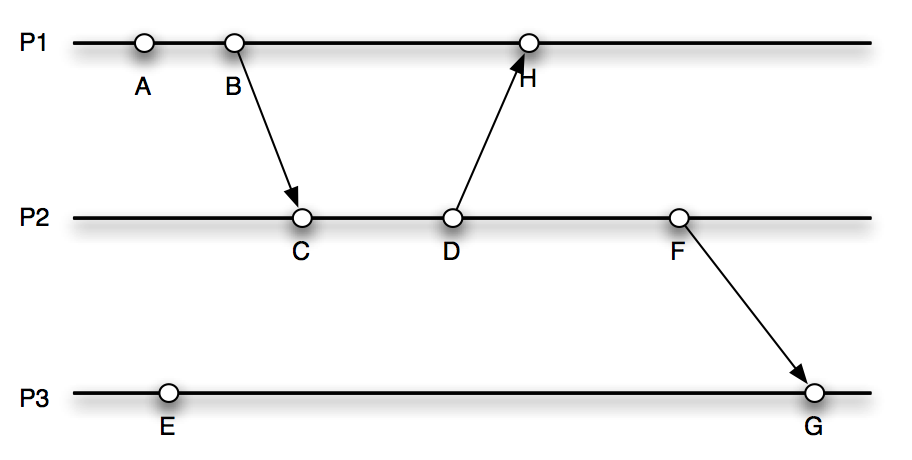
\includegraphics[width=0.5\textwidth]{Clocks.png}
\end{center}\end{figure*}

\begin{enumerate}
	\item Identify pairs of events that are logically concurrent. (In other words, in the absence of a global clock and tight time synchronization, which events cannot be distinguished as having occurred at different times?)
	\item Specify Lamport logical timestamps and vector clock timestamps for each event.
\end{enumerate}


%\item (It's party time!) You studied hard for your algorithms course, and to celebrate, you decided to throw a party for all VSP 2019 students. Some students, however, are not on good terms with others. You have a list of all $n$ students, along with information about whether any two students are not on good terms (conflicting). You would like to maximize the fun at the party, so you would like to minimize the number of pairwise conflicting students who are attending the party (no awkward encounters, please!) More precisely, you want to figure out the maximum number of students who are \emph{not} conflicting (pairwise), and, toward that end, you create a graph where each node represents a student, and an edge exists between two nodes iff the two corresponding students are not on good terms. 
%
%Your numerous attempts at coming up with a polynomial-time algorithm to solve this problem were not fruitful, so---because you are so eager to apply what you learned in class---you ignore organizing the party altogether and you set out to prove that this problem is $\textbf{NP}$-Complete.   
%
%  \begin{enumerate}
%  \item Let $\texttt{PARTY} \subset \{0,1\}^{*}$ denote the language corresponding to your problem. Write down \texttt{PARTY} precisely in terms of the graph abstraction described above. Note that we are concerned here with the \emph{decision} version of the problem: A problem whose possible answers are either \texttt{yes} or \texttt{no}. \\
%
%
%\item Show that $\texttt{PARTY} \in \textbf{NP}$. Describe both the certificate and the verifier program carefully. \\
%
%Recall the definition of the complexity class $\textbf{NP}$: A language $L \subseteq \{0,1\}^{*}$ is in $\textbf{NP}$ if there exists a polynomial $p:\mathbb{N} \to \mathbb{N}$ and a polynomial-time program (Turing machine) $M$ such that for every $x \in \{0, 1\}^{*}$,
%\begin{align*}
%x \in L \Longleftrightarrow \exists u \in \{0,1\}^{p(|x|) } \text{ s.t. } M(x,u) = \texttt{yes}.
%\end{align*}
%
%If $x \in L$ and $u \in \{0,1\}^{p(|x|)}$ satisfy $M (x,u ) = \texttt{yes}$, then we call $u$ a \emph{certificate} for $x$ (with respect to the language $L$ and machine $M$). Program $M$ is the \emph{verifier}. \\
%
%
%\item To finish off the $\mathbf{NP}$-Completeness proof, you need to show that \texttt{PARTY} is $\textbf{NP}$-Hard. Recall that a language $L'$ is $\textbf{NP}$-Hard if every language $L$ in $\mathbf{NP}$ is polynomial-time reducible to it. Language $L \subset \{0,1\}^{*}$ is \textbf{reducible} to $L' \subset \{0,1\}^{*}$ if there exists a polynomial-time computable function $f: \{0,1\}^{*} \to \{0,1\}^{*}$ such that $x \in L$ iff $f(x) \in L'$ (denoted $L \leq_{p} L')$. We showed in class that reductions are transitive (i.e., if $L_{1} \leq_{p} L_{2}$ and $L_{2} \leq_{p} L_{3}$, then $L_{1} \leq_{p} L_{3}$), so it is sufficient to pick one language that is known to be $\mathbf{NP}$-Complete and establish a reduction from it to our problem. We mentioned in class that the language \texttt{SAT} consisting of satisfiable Boolean formulae was the first language to be shown $\mathbf{NP}$-Complete (the Cook-Levin Theorem). Let $\varphi \equiv \varphi(x_{1}, \dotsc, x_{n})$ denote a Boolean formula on $n$ Boolean variables. An example is $\varphi = (x_{1}\vee x_{2} \vee \wbar{x}_{3})\wedge (x_{2} \vee x_{3})$, with 3 variables $x_{1}, x_{2}$, and $x_{3}$. A \textbf{satisfying assignment} for $\varphi$ is $x_{1}x_{2}x_{3}=101$. Formally,
%  \begin{align*}
%    \texttt{SAT} = \bigl\{\varphi: \varphi \text{ has a satisfying assignment} \bigr\}.
%  \end{align*}
%
%Define a \textbf{literal} to be either $x_{i}$ or $\wbar{x}_{i}$. A Boolean formula is in 3-Normal Conjunctive Form (3-CNF) if it is the conjunction (logical and) of clauses, each of which consisting of exactly 3 literals. An example of a Boolean formula in 3-CNF is $(x_{1}\vee x_{2} \vee \wbar{x}_{3})\wedge (x_{2} \vee x_{3} \vee \wbar{x}_{4})\wedge (x_{5} \vee \wbar{x}_{6} \vee \wbar{x}_{7}) \wedge (\wbar{x}_{5} \vee \wbar{x}_{8} \vee x_{9}) $; this formula has $4$ clauses (the expression in parenthesis), and each clause is the disjunction of exactly 3 literals. Define the language  
%\begin{align*}
%    \texttt{3SAT} = \bigl \{\varphi: \varphi \text{ is a satisfiable Boolean formula in 3-CNF} \bigr \}.
%  \end{align*}
%Convince yourself, but not the grader, that every Boolean formula can be converted to an equivalent 3-CNF formula in polynomial-time, and thus \texttt{3SAT} is \textbf{NP}-Complete. 
%
%
%We wish to show that $\texttt{3SAT} \leq_{p} \texttt{PARTY}$. Finding a satisfying assignment for a 3-CNF formula may be viewed as picking exactly one literal from each clause. However, the literals should be \textbf{consistent}, in the sense that the set of literals that you obtain after picking one from each clause should not contain a variable and its negation. For instance, in $(x_{1}\vee x_{2} \vee \wbar{x}_{3})\wedge (x_{2} \vee x_{3} \vee \wbar{x}_{4})\wedge (x_{5} \vee \wbar{x}_{6} \vee \wbar{x}_{7}) \wedge (\wbar{x}_{5} \vee \wbar{x}_{8} \vee x_{9})$, the set $\{x_{1}, x_{2}, \wbar{x}_{5}, \wbar{x}_{8}\}$ is consistent, and the corresponding assignment $x_{1}x_{2}x_{5} x_{8} = 1100$ (with any truth values assigned arbitrarily to any of the other variables) gives a satisfying assignment for this formula. The set $\{x_{1}, x_{2}, x_{5}, \wbar{x}_{5}\}$, on the other hand, is not consistent. Using this observation, for a given Boolean formula $\varphi$ consisting of $m$ clauses, construct a graph $G=(V, E)$ where each node is a literal that appears in $\varphi$ (if a literal appears in more than one clause, then it has a separate node in $G$ for each such occurrence) . An edge exists between two nodes in the graph if the corresponding literals are in the same clause in $\varphi$. Note that this edge forces all the literals in one clause to be in a separate connected component. However, the constraint that the literals you choose are consistent is not yet enforced in graph $G$. \emph{You are asked to complete the construction of graph $G$ by adding more edges to enforce the consistency constraint. After you are done, given a 3-CNF Boolean formula $\varphi = \varphi(x_{1}, \dotsc, x_{n})$ with $n$ variables and $m$ clauses, show that $\varphi \in \texttt{3SAT}$ if and only if graph $G$ that you constructed has at least $m$ students who are pairwise non-conflicting (on good terms). Argue that the transformation takes time that is polynomial in both the number of variables $n$ and the number of clauses $m$ of $\varphi$. Conclude that \texttt{PARTY} is \textbf{NP}-Complete.}
%
%\end{enumerate}
%
% \item Consider $n$ jobs $J_1, \dotsc, J_n$ that are all available for execution at time $0$, and that need to run on a multiprocessor platform. Once a job starts running on a processor, its execution cannot be interrupted. Job $J_i$ has execution time (length) $e_i \in \N$ and worst case (peak) memory requirement $M_i \in \N$ (in MB). Once assigned to processors, jobs cannot migrate to other processors (i.e., they keep running on the processor to which they are assigned until they finish execution). Moreover, the order of the jobs is fixed by the job dispatching system and so cannot be rearranged: \emph{In any allocation of processors to jobs, the jobs must appear in the same order as they are given in the input}. Assume that the jobs are ordered according to their indices such that $J_{1}$ is the first job to be dispatched for processing, and if $i<j$ and $J_{i}$ is assigned processor $k$, then job $J_{j}$ must either execute on processor $k$ and start after $J_{i}$, or execute on the $(k+1)$st processor. The processors onto which the jobs are to be partitioned are identical and 
% each has maximum available processing capacity (time) $L \in \N$; that is, the sum of execution times of the jobs assigned to any processor cannot exceed $L$. You may assume that $e_{i} \leqslant L$ for every $i \in \{1,\dotsc, n\}$.

% Given an allocation of processors to the input jobs, the peak memory demanded by processor $\pi_{j}$ under the given allocation is defined as $\max\{M_i: J_{i} \text{ is assigned to processor } \pi_{j}\}$. Our goal is to assign the jobs to as many processors as needed, respecting the given processor available time and the no rearrangement constraint, so that the overall peak memory usage is minimized; that is, the sum of the peak memory used on all processors is kept at a minimum. Develop an algorithm to solve this problem optimally and prove its correctness. Your algorithm should run in time $O(n^{2})$.

% \textbf{HINT:} Convince yourself, but not the grader, that the greedy algorithm that stuffs each processor as full as possible does not always give the minimum overall peak memory usage. An example exists. \\

% \textbf{Solution.} We will do this with dynamic programming. Think about the way in which the jobs are placed on the processor. We can iteratively place the jobs on the processor where, at each step, we can make a decision to either place the job on the current processor, or to open a new processor. Sometimes, of course, we will have no choice: The processor may not be able to fit the job, and we would then be forced to open a new processor.
% We will solve this problem first by going backwards. We will loop from $n$ down to 1 and determine the cheapest way (in terms of memory) of placing jobs $i$ through $n$ if we start a new processor with job $i$. We store the best costs in an array $\texttt{cost}$, where $\texttt{cost}[i]$ is the best possible memory cost of placing jobs $i$ through $n$. The recursion is the following:
% \begin{align*}
%   \texttt{cost}[i] = \min_{1 \leqslant k \leqslant m}\bigl \{ \texttt{cost}[i+k] + \max\{M_{i}, \dotsc, M_{i+k-1}\} \bigr\},
% \end{align*}
% where $m$ is the maximum integer such that $\sum_{j=i}^{m}e_{j} \leqslant L$. The base case is $\texttt{cost}[n]=M_{n}$. This recurrence can be converted to an iterative algorithm that runs in time $O(n^{2})$, which is \emph{strongly} polynomial.

\end{enumerate}



%%%%%%%%%%%%%%%%%%%%%%%%%%%%%%%%%%%%%%%%%%%%%%%%%%%%%%%%%%%%%%%%%%%%%%%%%
%% the bibliography starts here.

%\newpage
%\bibliographystyle{acm}
%\setlength{\baselineskip}{0.8\baselineskip}
%\bibliography{../../Bibliography/CompleteBibliography}

%%%%%%%%%%%%%%%%%%%%%%%%%%%%%%%%%%%%%%%%%%%%%%%%%%%%%%%%%%%%%%%%%%%%%%%%%
%% other closing material

% \appendix
% \input{appendix.tex}

\end{document}
%%% Local Variables:
%%% mode: latex
%%% TeX-master: t
%%% End:
